\documentclass[9pt]{beamer}
\usepackage{etex}
\usepackage{pres}
\usepackage{gensymb}

\makeatletter
\newif\if@restonecol
\makeatother
\let\algorithm\relax
\let\endalgorithm\relax
\usepackage[ruled,vlined,linesnumbered,lined]{algorithm2e}

\usefonttheme[onlymath]{serif}

\newcommand{\sseq}[1]{{\color{blue}\seq{#1}}}

\newcommand{\poly}{\textrm{poly}}
\newcommand{\Rat}{\mathbb{Q}}

\providecommand{\DontPrintSemicolon}{\dontprintsemicolon}

\pgfdeclareimage[width=6cm]{cps}{cps}
\pgfdeclareimage[width=6cm]{wsha}{wsha}
\pgfdeclareimage[width=6cm]{hybridA}{hybridAutomata}


\pgfdeclareimage[width=4cm]{hvac}{hvacs}
\pgfdeclareimage[width=3.1cm]{batt1}{batt}
\pgfdeclareimage[width=3.1cm]{batt2}{base}
\pgfdeclareimage[width=3.1cm]{batt3}{peak}

\pgfdeclareimage[width=11cm]{caro}{car}

\pgfdeclareimage[width=6cm]{geom1}{geom1}
\pgfdeclareimage[width=6cm]{geom2}{geom2}
\pgfdeclareimage[width=6cm]{geom3}{geom3}
\pgfdeclareimage[width=6cm]{geom4}{geom4}
\pgfdeclareimage[width=6cm]{geom5}{geom5}
\pgfdeclareimage[width=6cm]{geom6}{geom6}
\pgfdeclareimage[width=6cm]{geom7}{geom7}

\pgfdeclareimage[width=12cm]{bnd1}{boundarySch}
\pgfdeclareimage[width=12cm]{bnd2}{boundarySch1}
\pgfdeclareimage[width=12cm]{bnd3}{boundarySch2}
\pgfdeclareimage[width=12cm]{bnd4}{boundarySch3}

\pgfdeclareimage[width=4cm]{thumbreach}{thumbreach}


\hypersetup{
  pdftitle={Formal Verification: Projects},
  pdfauthor={Umang Mathur}}

\title{Solving Geometry Problems for Analysis of Cyber-Physical Systems}
\author{Umang Mathur \and Atul Sandur}
  

\institute[CS, UIUC] {\vspace{0.1cm} 
  Department of Computer Science\\
  University of Illinois, Urbana Champaign} 

  
\date{\today}

%%%%%%%%%%%%%%%%%%%%%%%%%%%%%%%%%%%%%%%%%%%%%%%%%%%%%%%%%%%%%%%%%%%%%%%%%%%%%%%%%%%%%%%%%% 
%%    Main Body
%%%%%%%%%%%%%%%%%%%%%%%%%%%%%%%%%%%%%%%%%%%%%%%%%%%%%%%%%%%%%%%%%%%%%%%%%%%%%%%%%%%%%%%%%%

\begin{document}

\frame{\titlepage}

\frame{\frametitle{Outline}
\tableofcontents}

\section{Introduction}
 \frame{
  \frametitle{Cyber-Physical Systems (CPS)}
  \begin{itemize}
    \item Cyber-Physical systems are engineered systems that depend upon the integration of
        \begin{itemize}
            \item computational algorithms, and 
            \item physical components 
        \end{itemize}
    \vspace{0.25in}
    \item Diverse applications:
        \begin{itemize}
            \item Healthcare
            \item Aerospace, Aeronautics
            \item Chemical processes
            \item Transportation
            \item Energy sector
        \end{itemize}
  \end{itemize}
}
   

\frame{
  \frametitle{Cyber-Physical Systems (CPS)}
  \begin{center}
    \pgfuseimage{cps} 
  \end{center}
}

\frame{
  \frametitle{Hybrid Automata: Modelling, Analysis and Synthesis of CPS}
  \begin{itemize}
  \item
    Introduced by Alur et al. to model hybrid systems
  \item
    Quite expressive, but \blue{undecidable} verification (reachability)
    problems  
  \item
    Decidable subclasses exists, e.g.
    \begin{itemize}
    \item 
      \blue{Timed Automata} ({\footnotesize Alur, and Dill}),
    \item 
      \blue{Initialized Rectangular Hybrid automata} ({\footnotesize Henzinger
        et al.}), 
 %   \item 
 %     \blue{Multi-Mode Systems} ({\footnotesize Alur, Trivedi, Wojtczak})   
    \end{itemize}
    \item Most verification techniques rely on exhaustive exploration of state space using finite bisimulations
%  \item 
 %   \blue{Tool support}: \textsc{HyTech}, \textsc{PHAV}er, \textsc{Uppaal}
  \end{itemize}
  \pause
    \begin{figure}
  \begin{center}
    \scalebox{0.8}{
    \begin{tikzpicture}[->,>=stealth',shorten >=1pt,auto,semithick]
      \tikzstyle{every state}=[fill=blue!30,minimum size=3em,rounded rectangle]
      
      \node[state] at (0, 0) (m0) {$\begin{array}{c}
          \mbox{\bf Off} \\ \dot{T} = -0.1T \\ T \geq 18 \end{array}$};
      
      \node[state] at (7, 0) (m1) {$\begin{array}{c} \mbox{\bf On} \\ \dot{T} = 5-0.1T \\ T \leq 22 \end{array}$};
     % \pause
  
      \path (m0) edge[bend left] node {$T < 19$} (m1);
      
      
      \path (m1) edge[bend left] node {$T > 21$} (m0);
      %\path (m0) edge node[] {$x_2 > 0, b$} (m2);
      
      %\path (m2) edge node[] {$ x_1 < 22, c$} (m3);
      %\path (m1) edge node[] {$d$} (m3);
   
      %\path (m3) edge [loop above] node[] {$e$} (m3);
    \end{tikzpicture}
  }
\end{center}
\label{fig:sha}
  \caption{Modelling a smart heater as a Hybrid Automata} 
\end{figure}
 
}

\section{Verification and Testing of Hybrid Automata}
\frame{\tableofcontentscurrent}

\frame{
  \frametitle{Reachability in Hybrid Systems}
  Safety Critical Systems :
    \begin{itemize}
        \item Nuclear reactors
        \item Chemical plants
        \item Aeronautics/Automobiles
    \end{itemize}
    It is therefore important to have certain safety guarantees for such systems

    \vspace{0.2in}
    Checking reachability of certain states, thus, is a natural question to ask
    \begin{itemize}
        \item Can reach some error state ?
        \item How to reach ?
            \begin{itemize}
                \item input ?
                \item path ? (non-determinism)
            \end{itemize}
    \end{itemize}

    \vspace{0.2in}
    Other interesting applications:
    \begin{itemize}
        \item Motion planning
    \end{itemize}
        
%%  \begin{center}
%%    \scalebox{0.8}{  \begin{tikzpicture}[node distance=1cm]
      \node[loc,label=below:$m_1$] (p4) at (0,-2.5) {$\begin{matrix} \dot{T_1} =
          -2 \\ \dot{T_2} = 3 \end{matrix}$};
      \node[loc,label=below:$m_2$] (p5) at (3,-2.5){$\begin{matrix} \dot{T_1} = -1 \\ \dot{T_2} = -1 \end{matrix}$};
    \node[loc,label=below:$m_3$] (p6) at (6,-2.5){$\begin{matrix} \dot{T_1} = -1 \\ \dot{T_2} = 3 \end{matrix}$};
    \node[loc,label=below:$m_4$] (p7) at (0,-5) {$\begin{matrix} \dot{T_1} = 2 \\ \dot{T_2} = -2 \end{matrix}$};
    \node[loc,label=below:$m_5$] (p8) at (3,-5){$\begin{matrix} \dot{T_1} = 2 \\ \dot{T_2} = -1 \end{matrix}$};
    \node[loc,label=below:$m_6$] (p9) at (6,-5){$\begin{matrix} \dot{T_1} = 2 \\ \dot{T_2} = 3 \end{matrix}$};
  \end{tikzpicture}
}
%%  \end{center}
%%  
%%  \vfill
%%
%%  \blue{Safe Schedulability Problem:} Does there exist a \blue{switching schedule} using these \blue{modes}
%%    such that the temperatures stay in \blue{comfortable region}? 
}

\subsection{Example}

\frame{
    \frametitle{Robotic Motion Planning}
    
    \vspace{-0.2in}
    \begin{figure}%{l}{0pt}%[0.4\textwidth]
\begin{center}
  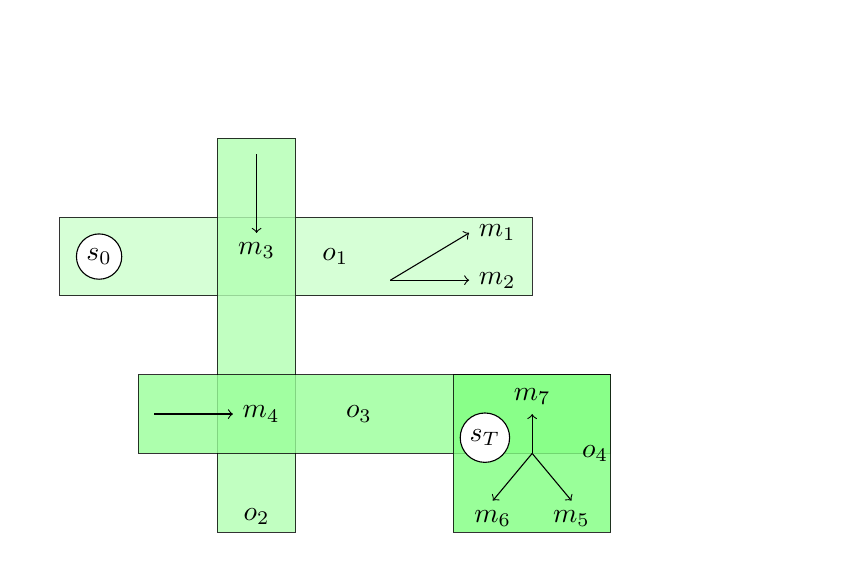
\begin{tikzpicture}
  \tikzstyle{every state}=[fill=gray!20!white,shape=rounded rectangle]
  
    \draw [fill=green!20, opacity=0.8] (0,0) rectangle (6,1);
    \node at (3.5, 0.5) {$o_1$};
    \node[fill=white!80, circle,inner sep=0.2em, draw] at (0.5, 0.5) {${\color{black}s_0}$};
    \draw[->] (4.2, 0.2) -- (5.2, 0.8) node[right] {$m_1$};
    \draw[->] (4.2, 0.2) -- (5.2, 0.2) node[right] {$m_2$};
    
    \draw [fill=green!30, opacity=0.8] (2,2) rectangle (3,-3);
    \node at (2.5, -2.8) {$o_2$};
    \draw[->] (2.5, 1.8) -- (2.5, 0.8) node[below] {$m_3$};
    
    \draw [fill=green!40, opacity=0.8] (1, -1) rectangle (7, -2);
    \node at (3.8, -1.5) {$o_3$};
    \draw[->] (1.2, -1.5) -- (2.2, -1.5) node[right] {$m_4$};
    
    \draw [fill=green!50, opacity=0.8] (5, -1) rectangle (7, -3);
    \node at (6.8, -2) {$o_4$};
    \draw[->] (6, -2) -- (6.5, -2.6) node[below] {$m_5$};
    \draw[->] (6, -2) -- (5.5, -2.6) node[below] {$m_6$};
    \draw[->] (6, -2) -- (6, -1.5) node[above] {$m_7$};
    \node[fill=white,circle,inner sep=0.2em, draw] at (5.4, -1.8)
    {${\color{black}s_T}$};
    
	\draw [dashed, draw=white] (6.6, 1.4) rectangle (7.4, -0.4);
    \draw [dashed, draw=white] (2.1, 3.4) rectangle (2.9, 2.6);
    \draw [dashed, draw=white] (-0.4, -1.1) rectangle (0.4, -1.9);
	\draw [dashed, draw=white] (7.6, -2.9) rectangle (9.9, -1.1);
      
    
    

  \end{tikzpicture}                        
\end{center}
  \caption{Robotic motion planning problem: Arena and feasible modes}
  \label{fig:robocop}
\end{figure}


    \begin{itemize}
        \item Can a bot enter $o4$ starting from some point in region $o1$ 
    \end{itemize}
}


\section{Singular Hybrid Automata: Syntax and Semantics}

\frame{
	\frametitle{Syntax of SHA}
	A singular hybrid automaton is a tuple \blue{$\Hh = (M, M_0, \Sigma, X, \Delta, I, F)$}
	where
	\begin{itemize}
		\item $M$ is a finite set of control {\color{blue}{modes}} and $M_0 \subseteq M$, 
		\item $\Sigma$ is a finite set of {\color{blue}actions},
		\item $X$ is an (ordered) set of {\color{blue}variables}, 
		\item $\Delta \subseteq M \times \poly(X) \times \Sigma \times 2^{X} \times M$ is the {\color{blue}transition relation}, 
		\item $I: M \to \poly(X)$  is the {\color{blue}mode-invariant} function, and
		\item $F: M \to \Rat^{|X|}$ is the mode-dependent {\color{blue}flow function} characterizing the rate of each variable in each mode.
	\end{itemize}
	
}

\frame{
	\frametitle{Semantics of WSHA}
	\begin{itemize}
	\item A \blue{configuration} $(m, \nu)$ and a \blue{timed action} $(t, a)$ 
	\item A \blue{transition} $((m, \nu) (t, a) (m', \nu'))$
	\begin{itemize}
		\item time elapse of $t$ in mode $m$ starting from $\nu$, followed by discrete step $a$
		\item guards, resets, invariants
	\end{itemize} 
	\item A \blue{run} is a sequence of transitions $(m_0, \nu_0) (t_1, a_1)
	(m_1, \nu_1) (t_2, a_2) \cdots$
	\end{itemize}
	
	\pause

	\begin{itemize}
	\item \blue{Type} $\Gamma(r)$ of a finite run 
	$r = \seq{(m_0, \nu_0), (t_1, a_1), (m_1, \nu_1), \ldots, (m_k, \nu_k)}$
	is a sequence 
	$\seq{n_0, b_1,  n_1,\ldots, b_p, n_p}$ defined as: 
	\begin{eqnarray*}
	  \Gamma(r) = 
	\begin{cases}
	  \seq{\varrho(m_0)} & \text{ if $r = \seq{(m_0, \nu_0)}$}\\
	  \Gamma(r') \oplus (a, \varrho(m)) & \text{ if $r = r'::\seq{(t, a), (m, \nu)}$},
	\end{cases}
	\end{eqnarray*}  

	\pause

	\item Any run (finite/infinite) will only have a \blue{finite run type}: there are only finitely many connected components,
	all sharing a partial order
	\end{itemize}
}



\frame{
  \frametitle{Formal Definitions}
  \begin{definition}[Constant-Rate Multi-Mode Systems: CMS]
    A CMS is a tuple $\Hh = (M, n, R)$
    where 
    \begin{itemize}
    \item $M$ is a finite nonempty set of \blue{modes}, 
    \item $n$ is the number of \blue{continuous variables}, 
    \item $R: M \to \Real^n$ gives for each mode
      the \blue{rate vector},
    \item $S \subseteq \Real^n$ is a \blue{bounded convex} set of \blue{safe states}.  
    \end{itemize}
  \end{definition}      
  \vfill
  \frametitle{Definition}
  \begin{block}{Safe Schedulability Problem}
    Given a \blue{multi-mode system} and a starting state,  decide whether there
    exists a \blue{non-Zeno safe schedule}.
  \end{block}
 % \pause
  \begin{block}{Safe Reachability Problem}
    Given a \blue{multi-mode system},  a \blue{starting state} and a \blue{target
      state}, decide whether there exists a safe schedule from starting
    state to target state.
  \end{block}
}

\frame{
  \frametitle{Key Results}

  \begin{theorem}[Alur et. al., 2011]
      Safe schedulability can be solved in \blue{polynomial time}. 
  \end{theorem}
  
  \begin{theorem}[Alur et. al., 2011]
      Safe reachability problem can be solved in \blue{polynomial time} if both
      starting and target states are in the interior of safety set.
  \end{theorem}
  
  \vspace{0.4in}
  Both the problems essentially boil down to solving a \blue{linear program} polynomial in size of the inputs.
  %Remark: 
  %A very special subclass of Hybrid automata, but the problems we consider
  %are \blue{undecidable} for Hybrid automata.
}



\frame{
  \frametitle{Safe Schedulability Problem}
  \begin{theorem}[Alur et. al]
    Assume that the starting state lies in the \blue{interior} of the safety set.  \\   
    
    A safe \blue{non-Zeno} schedule exists if and only if
    \begin{eqnarray*}
      \sum_{i=1}^{|M|} R(i) \cdot f_i &=& 0\\
      \sum_{i=1}^{|M|} f_i &=& 1.
    \end{eqnarray*}
    for some $f_1, f_2, \ldots, f_{|M|} \geq 0$.

    Moreover, such a schedule is \blue{periodic}.
  \end{theorem}
}

\frame{
  \frametitle{Safe Reachability Problem}
  \begin{theorem}[Alur et. al]
    Assume that the \blue{starting} state $s_0$ and the \blue{target} state
    $s_t$ lie in the \blue{interior} of the safety set. 
    
    A safe schedule exists from $s_0$ to $s_t$ exists if and only if 
    \begin{eqnarray*}
      s_0 + \sum_{i=1}^{|M|}  R(i) \cdot t_i  = s_t 
    \end{eqnarray*}
    for some  $t_1, t_2, \ldots, t_{|M|} \geq 0$. 
  \end{theorem}
}

\frame{
  \frametitle{Points to Remember: Schedulability}
  \begin{columns}
    \column{2in}
    The following is \blue{feasible}:
    \[    
    \sum_{i=1}^{|M|} R(i) \cdot f_i = 0  \text{ and  }\sum_{i=1}^{|M|} f_i = 1
    \]    
    Or, the following in \blue{infeasible}:
    \[
    (v_1, v_2, \ldots, v_n) \cdot R(i) > 0 \text{ for all modes $i$}.
    \]    
    \column{2in}
    \only<1>{{\small
  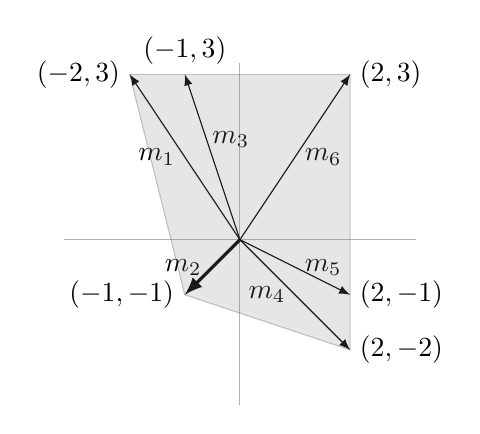
\begin{tikzpicture}[node distance=2cm,scale=0.7]
    \tikzstyle{lines}=[draw=black!30,rounded corners]
    \tikzstyle{vectors}=[-latex, rounded corners]
    \tikzstyle{rvectors}=[-latex,very thick, rounded corners]
    \draw[lines] (-3.2,0)--(3.2,0);
    \draw[lines] (0, 3.2)--(0,-3);
    \draw[vectors] (0, 0) --node[left]{$m_1$} (-2, 3) node[left]{$(-2,3)$};
    \draw[vectors] (0, 0) --node[left]{$m_4$} (2, -2)node[right]{$(2,-2)$};
    \draw[vectors] (0, 0) --node[right]{$m_6$} (2, 3)node[right]{$(2,3)$};
    \draw[rvectors] (0, 0) --node[left]{$m_2$} (-1, -1)node[left]{$(-1,-1)$};
    \draw[vectors] (0, 0) --node[above]{$~~~~m_3$} (-1, 3)node[above]{$(-1,3)$};
    \draw[vectors] (0, 0) --node[right]{$m_5$} (2, -1)node[right]{$(2,-1)$};

    \draw[fill=black!50,opacity=0.2] (-2,3) -- (-1,3) -- (2,3) --(2, -1) --(2,-2)
    -- (-1, -1) -- (-2, 3);
    
    
  \end{tikzpicture}
}
}
    \only<2>{{\small
  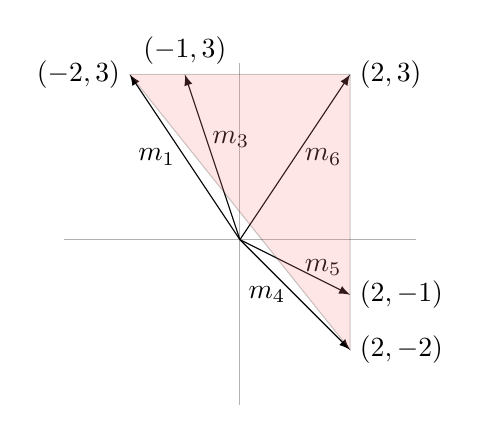
\begin{tikzpicture}[node distance=2cm,scale=0.7]
    \tikzstyle{lines}=[draw=black!30,rounded corners]
    \tikzstyle{vectors}=[-latex, rounded corners]
    \tikzstyle{rvectors}=[-latex,very thick, rounded corners]
    \draw[lines] (-3.2,0)--(3.2,0);
    \draw[lines] (0, 3.2)--(0,-3);
    \draw[vectors] (0, 0) --node[left]{$m_1$} (-2, 3) node[left]{$(-2,3)$};
    \draw[vectors] (0, 0) --node[left]{$m_4$} (2, -2)node[right]{$(2,-2)$};
    \draw[vectors] (0, 0) --node[right]{$m_6$} (2, 3)node[right]{$(2,3)$};
    \draw[vectors] (0, 0) --node[above]{$~~~~m_3$} (-1, 3)node[above]{$(-1,3)$};
    \draw[vectors] (0, 0) --node[right]{$m_5$} (2, -1)node[right]{$(2,-1)$};

    \draw[fill=red!50,opacity=0.2] (-2,3) -- (-1,3) -- (2,3) --(2, -1) --(2,-2)
     -- (-2, 3);
    
    
  \end{tikzpicture}
}
}
  \end{columns}
}

\frame{
  \frametitle{Points to Remember: Reachability}
  \begin{columns}
    \column{2in}
    The following is \blue{feasible}:
    \[    
    s_0 + \sum_{i=1}^{|M|}  R(i) \cdot t_i  = s_t 
    \]    
    \column{2in}
    \pgfuseimage{thumbreach}
  \end{columns}
}




\section{Weak Singular Hybrid Automata}
 \frame{\tableofcontentscurrent}

\frame{
	\frametitle{Motivation}
	\begin{center}
		\pgfuseimage{wsha}
	\end{center}
	
	\begin{itemize}
	\item Restricted mode switching
	\item Non-convex safety sets
	\item Decidable reachability (NP-complete), schedulability (NP-Complete), and
	LTL model-checking (PSPACE-complete) problems 
	\end{itemize}
}

\subsection{Example}

\frame{
    \frametitle{Robotic Motion Planning}
    
    \begin{figure}%{l}{0pt}%[0.4\textwidth]
\begin{center}
  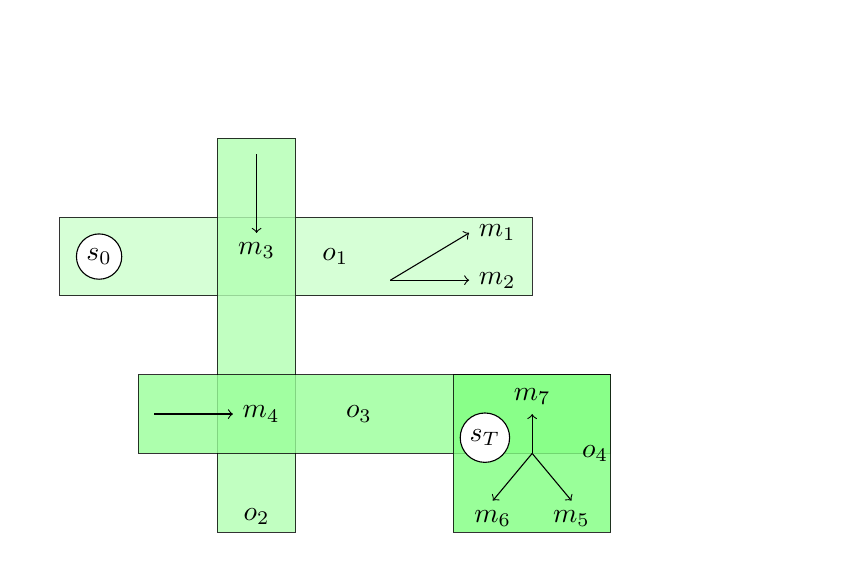
\begin{tikzpicture}
  \tikzstyle{every state}=[fill=gray!20!white,shape=rounded rectangle]
  
    \draw [fill=green!20, opacity=0.8] (0,0) rectangle (6,1);
    \node at (3.5, 0.5) {$o_1$};
    \node[fill=white!80, circle,inner sep=0.2em, draw] at (0.5, 0.5) {${\color{black}s_0}$};
    \draw[->] (4.2, 0.2) -- (5.2, 0.8) node[right] {$m_1$};
    \draw[->] (4.2, 0.2) -- (5.2, 0.2) node[right] {$m_2$};
    
    \draw [fill=green!30, opacity=0.8] (2,2) rectangle (3,-3);
    \node at (2.5, -2.8) {$o_2$};
    \draw[->] (2.5, 1.8) -- (2.5, 0.8) node[below] {$m_3$};
    
    \draw [fill=green!40, opacity=0.8] (1, -1) rectangle (7, -2);
    \node at (3.8, -1.5) {$o_3$};
    \draw[->] (1.2, -1.5) -- (2.2, -1.5) node[right] {$m_4$};
    
    \draw [fill=green!50, opacity=0.8] (5, -1) rectangle (7, -3);
    \node at (6.8, -2) {$o_4$};
    \draw[->] (6, -2) -- (6.5, -2.6) node[below] {$m_5$};
    \draw[->] (6, -2) -- (5.5, -2.6) node[below] {$m_6$};
    \draw[->] (6, -2) -- (6, -1.5) node[above] {$m_7$};
    \node[fill=white,circle,inner sep=0.2em, draw] at (5.4, -1.8)
    {${\color{black}s_T}$};
    
	\draw [dashed, draw=white] (6.6, 1.4) rectangle (7.4, -0.4);
    \draw [dashed, draw=white] (2.1, 3.4) rectangle (2.9, 2.6);
    \draw [dashed, draw=white] (-0.4, -1.1) rectangle (0.4, -1.9);
	\draw [dashed, draw=white] (7.6, -2.9) rectangle (9.9, -1.1);
      
    
    

  \end{tikzpicture}                        
\end{center}
  \caption{Robotic motion planning problem: Arena and feasible modes}
  \label{fig:robocop}
\end{figure}

}

\frame{
    \frametitle{Robotic Motion Planning}
    
    \begin{figure}%{l}{0pt}%[0.4\textwidth]
\begin{center}
  \begin{tikzpicture}
  \tikzstyle{every state}=[fill=gray!20!white,shape=rounded rectangle]
  
    \draw [fill=green!20, opacity=0.8] (0,0) rectangle (6,1);
    \node at (3.5, 0.5) {$o_1$};
    \node[fill=white!80, circle,inner sep=0.2em, draw] at (0.5, 0.5) {${\color{black}s_0}$};
    \draw[->] (4.2, 0.2) -- (5.2, 0.8) node[right] {$m_1$};
    \draw[->] (4.2, 0.2) -- (5.2, 0.2) node[right] {$m_2$};
    
    \draw [fill=green!30, opacity=0.8] (2,2) rectangle (3,-3);
    \node at (2.5, -2.8) {$o_2$};
    \draw[->] (2.5, 1.8) -- (2.5, 0.8) node[below] {$m_3$};
    
    \draw [fill=green!40, opacity=0.8] (1, -1) rectangle (7, -2);
    \node at (3.8, -1.5) {$o_3$};
    \draw[->] (1.2, -1.5) -- (2.2, -1.5) node[right] {$m_4$};
    
    \draw [fill=green!50, opacity=0.8] (5, -1) rectangle (7, -3);
    \node at (6.8, -2) {$o_4$};
    \draw[->] (6, -2) -- (6.5, -2.6) node[below] {$m_5$};
    \draw[->] (6, -2) -- (5.5, -2.6) node[below] {$m_6$};
    \draw[->] (6, -2) -- (6, -1.5) node[above] {$m_7$};
    \node[fill=white,circle,inner sep=0.2em, draw] at (5.4, -1.8)
    {${\color{black}s_T}$};

    \pause
    
	\node[state,fill=gray!20, scale=0.7] at (7, 1) (m1) {$m_1$};
	\node[state,fill=gray!20, scale=0.7] at (7, 0) (m2) {$m_2$};
	\draw [dashed] (6.6, 1.4) rectangle (7.4, -0.4);
	\path[->] (m1) edge[bend left] (m2);
     \path[->] (m2) edge[bend left] (m1);
	
	\node[state, fill=gray!20, scale=0.7] at (2.5,3) (m3) {$m_3$} ;
    \draw [dashed] (2.1, 3.4) rectangle (2.9, 2.6);
    
    \node[state, fill=gray!20, scale=0.7] at (0,-1.5) (m4) {$m_4$} ;
    \draw [dashed] (-0.4, -1.1) rectangle (0.4, -1.9);
    
	\node[state, fill=gray!20, scale=0.7] at (8,-1.5) (m5) {$m_5$} ;
	\node[state, fill=gray!20, scale=0.7] at (9.5,-1.5) (m6) {$m_6$} ;
	\node[state, fill=gray!20, scale=0.7] at (8.75,-2.5) (m7) {$m_7$} ;
	\draw [dashed] (7.6, -2.9) rectangle (9.9, -1.1);
	\path[->] (m5) edge (m6);
    \path[->] (m6) edge (m7);
    \path[->] (m7) edge  (m5);
      
    
    

  \end{tikzpicture}                        
\end{center}
  \caption{Robotic motion planning problem: Modelling as a SHA}
  \label{fig:robocop}
\end{figure}

}

\frame{
    \frametitle{WSHA: Robotic Motion Planning}
    
    \begin{figure}[t]

  \begin{center}
     \scalebox{0.9}{
    \begin{tikzpicture}
      \tikzstyle{every state}=[fill=gray!20!white,minimum size=2em,shape=rounded rectangle]
      

      \node[state,fill=gray!20] (m1) {$m_1$};
      \node[state,fill=gray!20] at (0, -2) (m2) {$m_2$};
      \draw [dashed] (-0.5, 0.5) rectangle (0.5, -2.5) node[right] {$o_1$};
      \node at (0, -2.8) {$0{<} x {<} 6$};
      \node at (0, -3.1) {$0 {<} y {<} 1$};
      
      
      \node[state, fill=gray!20] at (2.5,0) (m3) {$m_3$} ;
      \draw [dashed] (2, 0.5) rectangle (3, -0.5) node[right]{$o_2$} ;
      \node at (2.5, -0.8) {$2{<} x {<} 3$};
      \node at (2.5, -1.1) {$-3 {<} y {<} 3$};

      \node[state, fill=gray!20] at (5.5,0) (m4) {$m_4$} ;
      \draw [dashed] (5, 0.5) rectangle (6, -0.5) node[right]{$o_3$};
      \node at (5.5, -0.8) {$1{<} x {<} 7$};
      \node at(5.5, -1.1) {$-2 {<} y {<} {-}1$};

      \node[state, fill=gray!20] at (8,0) (m5) {$m_5$} ;
      \node[state, fill=gray!20] at (10,0) (m6) {$m_6$} ;
      \node[state, fill=gray!20] at (9,-2) (m7) {$m_7$} ;
      \draw [dashed] (7.5, 0.5) rectangle (10.5, -2.5) node[right]{$o_4$};
      \node at (9, -2.8) {$5 {<} x {<} 7, -3 {<} y {<} -1$};

     \path[->] (m1) edge[bend left] node [right] {$\top$}  (m2);
     \path[->] (m2) edge[bend left] node [left] {$\top$}  (m1);

     \path[->] (m1) edge node [above] {$2 {<} x {<} 3$}  (m3);
     \path[->] (m3) edge node [above] {$-2 {<} y {<} -1$}  (m4);

     \path[->] (m4) edge node [above] {$5 {<} x {<} 7$}  (m5);

    \path[->] (m5) edge node [above] {$\top$}  (m6);
    \path[->] (m6) edge node [right] {$\top$}  (m7);
    \path[->] (m7) edge node [left] {$\top$}  (m5);
    \end{tikzpicture}
    }
  \end{center}
\caption{Singular Hybrid Automaton for robotic motion planning example}
\label{fig:wsha}
\end{figure}


}

\subsection{Syntax and Semantics}

\frame{
	\frametitle{Syntax of WSHA}
	A weak singular hybrid automaton is a tuple \blue{$\Hh = (M, M_0, \Sigma, X, \Delta, I, F)$}
	where
	\begin{itemize}
		\item $M$ is a finite set of control {\color{blue}{modes}} and $M_0 \subseteq M$, 
		\item $\Sigma$ is a finite set of {\color{blue}actions},
		\item $X$ is an (ordered) set of {\color{blue}variables}, 
		\item $\Delta \subseteq M \times \poly(X) \times \Sigma \times 2^{X} \times M$ is the {\color{blue}transition relation}, 
		\item $I: M \to \poly(X)$  is the {\color{blue}mode-invariant} function, and
		\item $F: M \to \Rat^{|X|}$ is the mode-dependent {\color{blue}flow function} characterizing the rate of each variable in each mode.
	\end{itemize}
	
	\pause
	\vspace{0.2in}
	Function \blue{$\varrho: M \rightarrow \Nat$} assigning \blue{ranks} to the modes such that
	\begin{itemize}
		\item for every transition $(m, G, a, R, m') \in \Delta$, \blue{$\varrho(m) \leq \varrho(m')$}, and 
		\item for every rank $i$ the set of modes with rank $i$
		\begin{itemize}
			\item has a \blue{common safety set $S_i$} which is a bounded and open polytope (\blue{problems with boundaries})
			\item is \blue{strongly connected} with no resets or guards
		\end{itemize}
	\end{itemize}
}

\frame{
	\frametitle{Semantics of WSHA}
	\begin{itemize}
	\item A \blue{configuration} $(m, \nu)$ and a \blue{timed action} $(t, a)$ 
	\item A \blue{transition} $((m, \nu) (t, a) (m', \nu'))$
	\begin{itemize}
		\item time elapse of $t$ in mode $m$ starting from $\nu$, followed by discrete step $a$
		\item guards, resets, invariants
	\end{itemize} 
	\item A \blue{run} is a sequence of transitions $(m_0, \nu_0) (t_1, a_1)
	(m_1, \nu_1) (t_2, a_2) \cdots$
	\end{itemize}
	
	\pause

	\begin{itemize}
	\item \blue{Type} $\Gamma(r)$ of a finite run 
	$r = \seq{(m_0, \nu_0), (t_1, a_1), (m_1, \nu_1), \ldots, (m_k, \nu_k)}$
	is a sequence 
	$\seq{n_0, b_1,  n_1,\ldots, b_p, n_p}$ defined as: 
	\begin{eqnarray*}
	  \Gamma(r) = 
	\begin{cases}
	  \seq{\varrho(m_0)} & \text{ if $r = \seq{(m_0, \nu_0)}$}\\
	  \Gamma(r') \oplus (a, \varrho(m)) & \text{ if $r = r'::\seq{(t, a), (m, \nu)}$},
	\end{cases}
	\end{eqnarray*}  

	\pause

	\item Any run (finite/infinite) will only have a \blue{finite run type}: there are only finitely many connected components,
	all sharing a partial order
	\end{itemize}
}



\subsection{Reachability and Schedulability}

\frame{
	\frametitle{Reachability and Schedulability}
	
	\begin{theorem}
	  The reachability and schedulability problems for weak singular hybrid automata are NP-complete.
	\end{theorem}
	
	\begin{itemize}
		\item NP Hardness: \pause Reduction from Subset-sum problem (Reachability) .\pause
		\begin{figure}[t]
			\begin{center}
				\scalebox{0.5}{
					\begin{tikzpicture}[->,>=stealth',shorten >=1pt,auto,node distance=1.8cm, semithick]
						\tikzstyle{every state}=[fill=black!30!white,minimum size=3em,rounded rectangle]
						\node[state] at (1.7,1.5) (A0) {$\begin{array}{c}m_0 \\ (1,1,2,-3,0,0) \end{array}$} ;
						\node[state] at (0,0) (A1) {$\begin{array}{c}m_1 \\ (0,-1,0,0,1,1) \end{array}$} ;
						\node[state] at (0,-2) (B1) {$\begin{array}{c}m_3 \\ (0,0,-2,0,2,1) \end{array}$} ;
						\node[state] at (0,-4) (B2) {$\begin{array}{c}m_5 \\ (0,0,0,3,-3,1) \end{array}$} ;
						\node[state] at (4,0) (A) {$\begin{array}{c} m_2 \\ (0,-1,0,0,0,0) \end{array}$} ;
						\node[state] at (4,-2) (B) {$\begin{array}{c} m_4 \\ (0,0,-2,0,0,0) \end{array}$} ;
						\node[state] at (4,-4) (C) {$\begin{array}{c} m_6 \\ (0,0,0,3,0,0) \end{array}$} ;

						\path (A0) edge node [above]{} (A);
						\path (A0) edge node [above]{} (A1);
						\path (A1) edge node [above]{} (B);
						\path (A1) edge node [above]{} (B1);
						\path (A) edge node [above]{} (B);
						\path (A) edge node [above]{} (B1);
						\path (B1) edge node [above]{} (B2);
						\path (B1) edge node [above]{} (C);
						\path (B) edge node [above]{} (B2);
						\path (B) edge node [above]{} (C);
						
						%\node at (0,-5) (TEXT) {$\nu_0 = \vzero$, Target = ($1, [1,3], [1,3], [1,3]$, sum, $[1,3]$)};
					 \end{tikzpicture}
				}
				\caption{Constructed WSHA for set $\{1,2,-3\}$}
				\label{nphard}
			\end{center}
		\end{figure}
		\pause
		\item Schedulability: Reachability to the last strongly connected component and multi-mode scheduling there
	\end{itemize}

}

\frame{
	\frametitle{Reachability and Schedulability}
	
	\begin{itemize}
		\item NP-Membership: \pause
			\begin{itemize}
				\item All run-types are polynomial in size of the WSHA. \pause
				\item Checking whether a run type $\sigma = \seq{n_0, b_1, n_1, \ldots, b_p, n_p}$ is reachable/schedulable
				amounts to checking the feasibility of a linear program ($\nu_{n_i}, \nu_{n_i}' \in \Real^{|X|}$ and  $t_i^m \in \Rplus$ are variables): \pause
				\begin{flushleft}
					\scalebox{0.8}{
					\begin{columns}[t]
					\begin{column}{0.55\textwidth}
						\begin{eqnarray}
							\nu_0 &=& \nu_{n_0} \nonumber \\
							\nu_{n_p}' & \in & \Tt \nonumber\\
							\nu_{n_i}, \nu_{n_i}'  & \in & S_{M_{n_i}} \text{ for all $0 \leq i \leq p$} 
							\nonumber \\
							\nu_{n_i}   & \in & G(b_i) \text{ for all $0 < i \leq p$}
							\nonumber \\
							\nu_{n_{i+1}}(j) &=& 0 \text{ for all $x_j \in R(b_{i+1})$} \nonumber\\ & &\text{and }  0 < i \leq p
							\nonumber \\
							\nu_{n_{i+1}}(j) &=& \nu_{n_i}'(j)  \text{ for all} x_j \not \in R(b_{i+1}) \nonumber\\ & & \text{and } 0 < i \leq p
							\nonumber \\
							\nu_{n_i}'  & = & \nu_{n_i} + \sum_{m \in M_{n_i}} F(m) \cdot t_i^m \nonumber\\
							& &\text{ for all $0 \leq i \leq p$}\nonumber\\% \label{eqn-wsha-reach}\\
							t_i^m  &\geq&  0 \text{ for all $0 \leq i \leq p$ and  $m \in M_{n_i}$} \nonumber
						\end{eqnarray}
						\newline
						\\[2.4pt]
						{\large Linear program for Reachability}
					\end{column}
					\pause
					\begin{column}{0.6\textwidth}
						\begin{eqnarray}
							\nu_0 &=& \nu_{n_0} \nonumber \\
							\nu_{n_i}, \nu_{n_i}'  & \in & S_{M_{n_i}} \text{ for all $0 \leq i \leq p$}
							\nonumber \\
							\nu_{n_i}   & \in & G(b_i) \text{ for all $0 < i \leq p$}
							\nonumber \\
							\nu_{n_{i+1}}(j) &=& 0  \text{ for all $x_j \in R(b_{i+1})$ and  $0 < i \leq p$}
							\nonumber \\
							\nu_{n_{i+1}}(j) &=& \nu_{n_i}'(j)  \text{ for all $x_j \not \in R(b_{i+1})$ and  $0 < i \leq p$}
							\nonumber \\
							\nu_{n_i}'  & = & \nu_{n_i} + \sum_{m \in M_{n_i}} F(m) \cdot t_i^m \text{
							for all $0 \leq i \leq p$} \nonumber\\%\label{eqn:wsha-sched}\\
							t_i^m  &\geq&  0 \text{ for all $0 \leq i \leq p$ and $m \in M_{n_i}$} \nonumber\\ 
							\vzero &=& \sum_{m \in M_{n_p}} F(m) \cdot t_p^m  \nonumber\\
							1 &=& \sum_{m \in M_{n_p}} t_p^m \nonumber
						\end{eqnarray}
						\newline
						\\[1pt]
						{\large Linear program for Schedulability}
					\end{column}
				\end{columns}
				}
				\end{flushleft}
				
				
			\end{itemize}
	\end{itemize}
}

\subsection{Temporal Logic Model Checking}

\frame{
	\frametitle{Temporal Logic Model Checking}
	
	LTL Model Checking: Just the best !
	\begin{theorem}
		The LTL model-checking problem for WSHA is PSPACE-complete.
	\end{theorem}
	\pause
	\begin{itemize}
		\item LTL property $\phi$ $\to$ B\"uchi automata $\Aa_{\neg \phi}$ 
		\item Product of a WSHA $\Hh$ and $\Aa_{\neg \phi}$ remains
		WSHA (since variables occur only in the WSHA component).  
		\item Standard polynomial space algorithm can be used. 
		\item PSPACE-hardness of the problem follows from PSPACE-completeness of LTL model checking over a finite automaton
	\end{itemize}
	\vspace{0.2in}
	\pause
	CTL Model Checking: Not so easy !
	\begin{theorem}
		CTL model checking of weak SHAs with two variables is PSPACE-hard. 
	\end{theorem}
	\pause
	\begin{itemize}
		\item Polynomial reduction from subset-sum games
		\item Decidability: \blue{still open}
	\end{itemize}
}
\subsection{Extending WSHA}

\frame{
	\frametitle{WSHAs are JUST Decidable}
	WSHA is on the forefronts of decidability. Tweaking the model in the hope to improve expressiveness
	can lead to undecidability !

	\pause

	\begin{theorem}
		The reachability problem is undecidable for three variable WSHAs with discrete
		updates. 
	\end{theorem}
	 
	\pause 
	\begin{theorem}
		The reachability problem is undecidable for CMS with two variables and one
		unrestricted clock. 
	\end{theorem}
}

\section{Summary}

\frame{
	\frametitle{Summary and Future Work}
	\begin{itemize}
		\item WSHAs as a subclass of Hybrid automata. \pause
		\item Efficient model : Reachability, Schedulability and LTL Model Checking are Decidable \pause
		\item Slight extensions can lead to undecidability in results
	\end{itemize}

	\pause
	\begin{itemize}
		\item Future work
		\begin{itemize}
			\item Decidability of CTL Model Checking for this problem is still unsolved
			\item Games on WSHA and restrictions on WSHA
			\item CEGAR framework : Approximate modeling of undecidable subclasses of hybrid automata using WSHA (Ongoing)
		\end{itemize}
	\end{itemize}
}

\frame{
\frametitle{}
	\begin{center}

        \font\endfont = cmss9 at 15.40mm
        \endfont 
        \baselineskip 20.0mm

        Thank You !

      \end{center}    
}

\nocite{*}

\bibliographystyle{plain}
\bibliography{papers}

\end{document}
